\documentclass[journal]{IEEEtran}

\usepackage{mathtools}
\usepackage{amsmath}
\usepackage{amssymb}
\usepackage{graphicx}
\usepackage{epstopdf}
\usepackage{cite}
\usepackage{array}
\usepackage{eurosym}
\usepackage{balance}
\usepackage{url}

\usepackage{color}

\newcommand{\hilight}[1]{\colorbox{yellow}{#1}}


\newcommand{\highlight}[1]{%
  \colorbox{yellow}{$\displaystyle#1$}}

\hyphenation{op-tical net-works semi-conduc-tor mo-nitoring}
\newcommand\blfootnote[1]{%
  \begingroup
  \renewcommand\thefootnote{}\footnote{#1}%
  \addtocounter{footnote}{-1}%
  \endgroup
}

\begin{document}

\title{A Rectifier Circuit Insensitive  to the  Angle of Incidence of Incoming Waves Based on a Wilkinson Power Combiner}

\author{
\IEEEauthorblockN{Spyridon Nektarios Daskalakis,~\IEEEmembership{Student Member,~IEEE},
Apostolos Georgiadis,~\IEEEmembership{Senior Member,~IEEE}
George Goussetis,~\IEEEmembership{Senior Member,~IEEE}, 
and Manos M. Tentzeris,~\IEEEmembership{Fellow,~IEEE}}

%\vspace{-1cm}
\thanks{
Manuscript received Month DD, YYYY; revised Month DD, YYYY; accepted Month DD, YYYY.
This work was supported by Lloyd's Register Foundation (LRF) and the International Consortium in Nanotechnology (ICON).
%
The work of M. M. Tentzeris was supported by the National Science Foundation (NSF) and the Defense Threat Reduction Agency (DTRA).
%


This paper is an expanded version from the
2nd URSI Atlantic Radio Science Conference (URSI AT-RASC), Gran Canaria, 28 May - 1 June 2018.

S. N. Daskalakis, G. Goussetis and A. Georgiadis  are with School of Engineering \& Physical Sciences;  Institute of Sensors, Signals and Systems, Heriot-Watt University, Edinburgh, EH14 4AS, Scotland,
UK (e-mail: sd70@hw.ac.uk, g.goussetis@hw.ac.uk, apostolos.georgiadis@ieee.org).

M. M. Tentzeris is with School of Electrical and Computer Engineering, Georgia Institute of Technology, Atlanta, GA 30332-250, USA (e-mail: etentze@ece.gatech.edu).
}}




\maketitle

\begin{abstract}

%Radio Frequency (RF) energy harvesting, has been gaining interest over the last years because the  number of RF emitters have been increasing. 
%
%Broadcasting transmitters are widely used and there is an engineering challenge about how to collect the unused ambient RF energy and supply low-power  devices.
%
In this work a novel high efficiency, low-cost and low-complexity RF-to-dc converter was designed for  RF energy harvesting in the $2.4$~GHz band. 
%
The proposed design has two RF inputs and maintains a high efficiency over a wide range of  incoming incident wave angles.
%
The circuit is based on a Wilkinson power combiner and has two single-diode rectifiers. 
%
One rectifier is connected at the combiner's output  and 
collects the energy coming from the two inputs.
%
The second rectifier replaces the isolation resistor of the combiner in order to collect the power that would otherwise be dissipated in it.
%
The second rectifier is used for recycling the wasted power when the input signals do not have the same phase. 
%
The novel RF-to-dc converter was fabricated  using commercially available components and low-cost FR-4 substrate.
%
A prototype was designed and its efficiency was optimized for low power input levels.
%
The measured system efficiency
was $16.2 \%$ for in-phase input signals with available input power $-17$~dBm.
% 
When the relative phase of  input signals varied from $0$ to $360$ degrees, a variation in efficiency  between $15.3\%$  and $22\%$  was observed. 
%
For input power $3$~dBm, the efficiency varies from $26\%$  to   $39\%$ between $0$ to $360$ degrees phase difference.

\end{abstract}

\begin{IEEEkeywords}
Internet-of-Things (IoT), radio frequency (RF) energy harvesting,  radio frequency identification (RFID), rectifier, Wilkinson divider, wireless power transfer.
\end{IEEEkeywords}


\IEEEpeerreviewmaketitle



\section{Introduction}

\IEEEPARstart{I}{n} our days  radio frequency (RF) energy harvesting is an atractive way to capture power in  conditions where  light or wind sources are not available \cite{shinohara2011power,  pinuela2013ambient, niotaki2014solar, kim2014ambient}. 
%
Broadcasting RF transmitters like FM/TV, cellular networks base stations, WiFi routers, and frequency identification (RFID) readers, have been increasing rapidly around us, due to the huge development of  wireless technologies.
%
In 1964 William C. Brown proposed  a system for transformation of RF power to dc power  \cite{brown1984history}. 
%
In this  RF-to-dc converter, an antenna is combined with a rectifier, which  consists of one or more diodes in specific configuration, forming a rectenna.
%
One significant  limitation in  rectenna design is
the relatively low available ambient power density level as well as the RF-to-dc power efficiency of the circuit \cite{valenta2014harvesting,kim2014ambient}.
%
%Several selected challenges related to developing RF energy harvester are discussed in \cite{daskalakis2016dual, collado2017rectifier, kimionis2017octave, daskalakis2017uhf}.
%
%It is coved the  designs  of  multiband  and  broadband  rectifiers and the  minimization  of  the  effect  that  load  and  input  power  variations  have  on  the  system  performance.
%
It remains an engineering challenge how to capture unused ambient RF energy and use it to supply small sensor nodes, such as radio frequency identification (RFID) tags \cite{kim2014ambient, assimonis2015sensitive, kotani2009high}.
%RFIDs have become a highly desirable technology  for sensing applications \cite{daskalakis2017ambient}.
%
%The tags use embedded rectennas in order to capture the energy for the communication with the reader.
%
%Existing passive RFID technology is mostly limited to only identifying and inventorying items placed near the reader, so the design of  tags and thus rectennas  placed at  far-field, is something necessary for future applications. 
%
Interest in Internet of Things (IoT) low-power sensors powered by RF ambient power or wireless power transmission has increased due to the vision of ubiquitous sensing as part of 5G mobile networks.
%
Wireless powering in the $2.4$~GHz  industrial, scientific and medical  (ISM) band can enable
applications where a large number of mobile devices with WiFi/Bluetooth transceivers can act as RF sources to power the  sensors. 
%
%Approaches to improve the rectifier sensitivity in the prior art include novel rectifier topologies to reduce current loads during the charging phase \cite{kang201621}. 

%
%As the fifth generation (5G) standardization is in on-going phase, one of the most used terminology in next generation systems will be the word ``Green''.
%
In most 5G industrial visions, the high energy efficient   ``Green'' performance for 5G systems is pointed out as a necessity both for devices and networks. 
%
Consequently RF energy harvesting seems to be a very promising technique for future 5G ``Green'' systems.
%
In this case, nearby relays are considered which  include wireless power transfer capabilities  together with the RF communication signals.
%
Millimeter-wave (mmWave) signals could deliver both information and energy to the end  small devices, like next generation RFIDs \cite{kimionis2017millimeter, tong2019achieving}. 
%
Such, an RFID device, capable of operating autonomously and with a reading range of  tens  of meters, would provide a very effective interface point between the IoT and 5G networks
\cite{hester2017mm}.


 




This paper addresses the problem of RF versus dc power combining in rectenna array systems.
%
Increasing the number of antennas and therefore the effective area available for collection of RF energy is a straightforward approach in order to increase the total RF energy that is being harvested. Due to the nonlinear nature of the rectifier circuit however, when the RF energy which is being available to the individual rectenna element is very small, the RF-to-dc conversion efficiency of the rectifier is also very small leading to a non-optimal performance. 
%
Therefore, not only the overall number of rectenna elements but the RF power available to each element is important in order to maximize the system  efficiency and ultimately the dc output power. 
%
As a result, one might first consider rectenna elements where one rectifier is connected to an antenna array thereby achieving superposition of RF energy before the RF-to-dc conversion. 
%
For example in \cite{marshall2013staggered},
the concept of an $N \times N$ staggered pattern charge collector (SPCC) is described  in order to achieve maximum energy harvesting efficiency. 
%
%The SPCC consists of $N$ sub-arrays that contain N antenna elements and each sub-array is connected to an energy harvester circuit. 
%
%All the energy harvesters are connected on one capacitor or load. 
%
%The proposed setup uses multiple antennas sub-arrays with phase offsets and thus the main beams have not only high gain but a larger beamwidth than a single array.  
%
%Each sub-array is designed to aim in different directions and cover the same area as a single antenna.
%
Using the above consent, more energy harvesters and thus more diode elements are used in order to cover a wideband area.
%
Another disadvantage of this topology is that superposition of RF energy corresponds to directive antenna elements and one is not able to harvest RF energy coming from different angular directions but only from selected angular directions where the antenna array gain is maximized. 

\begin{figure}[t]
\centering
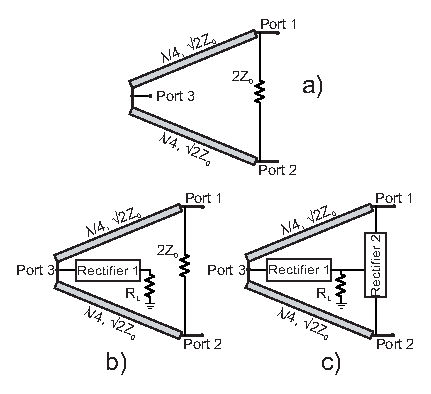
\includegraphics[width=0.8\columnwidth]{Figures/Fig1.eps}
\caption{Power combiner circuits with rectification capabilities. a) Typical Wilkinson combiner circuit.    
b) Wilkinson combiner circuit with single rectifier c) Wilkinson combiner  with two rectifier circuits. One rectifier has been installed at the port  $3$ and the isolation resistor has been replaced with a second rectifier.}
\label{fig:1}
\end{figure}

One way around this problem is to employ beam-steering
architectures but such systems consume energy in steering the
antenna beam and therefore one needs to take into account
the amount of energy spent in the beam steering process in
order to compute the overall RF-to-dc conversion efficiency
of the system. 
%
A different approach is to design a sub-array topology where each sub-array is pointed to a fixed
but different angular direction.
%
 This way one achieves a
high efficiency at a fixed predetermined number of angular
directions and a  good overall efficiency for a range of angular directions
at the expense of an increased complexity in the antenna 
\cite{lee2017hybrid}.
%


In this work we demonstrate a scalable, two branch rectifier which is capable of maintaining a constant RF-to-dc conversion efficiency over any phase shift between the RF
signals present at its input terminals, and therefore over any
angular direction.
%
This topology
is able to combine RF energy from any angular direction
and convert it efficiently to dc output power. It is based on
a Wilkinson power combiner and it is scalable, employing
combiner modules connected to a large number of antenna
elements or sub-arrays and subsequently combining the output
in series or parallel configuration.


In addition to RF power combining our rectifier employs dc power combining at $2.4$~GHz by optimally combining the output of two rectifiers in parallel. 
%
 Our rectifier design could be easily scaled up to mmWave frequencies (i.e. $60$~GHz) and miniaturized for a future 5G application.  
%
Therefore we propose a rectifier module which provides RF and dc power combining to achieve a high conversion efficiency with minimum variation from RF signals with arbitrary phase, thereby utilizing a nonlinear device to maintain both a high gain and an omnidirectional characteristic for a rectenna.
%



\begin{figure}[t]
\centering
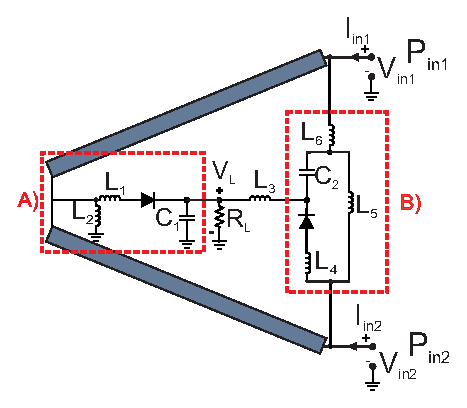
\includegraphics[width=0.8\columnwidth]{Figures/Fig2.eps}
\caption{Circuit of the double design. Two single rectifiers (dash rectangle) have been combined using a common load $R_\text{L}$.}
\label{fig:2}
\end{figure}

Some research efforts have been made in harvesting
using Wilkinson combiners or dividers. 
%
In \cite{olgun2010low}, a rectenna design is proposed and integrated with RFID sensors to harvest ambient power from the RF devices operating in the $2.4$~GHz ISM band.
%
The circuit consists of two diode pairs, a Wilkinson power divider, storage and bypass capacitors and an impedance matching circuit.
%
Measured performance for the rectifier is given and shown to be $70\%$ efficient for high power signals of $3$~dBm.
%
In  \cite{alneyadi20142}, the researchers present results of an RF energy harvester at $2.4$~GHz WiFi-WLAN frequency band. 
%
A Wilkinson's circuit is used to combine the RF signals from two patch antennas and supply a modified Greinacher rectifier. 
%
This dc energy is stored in a super capacitor in order to
supply on-demand self-powered sensor nodes.
%
The maximum efficiency is measured to be $57.8\%$ at $6$~dBm  input power. 
%
%In the presence of a realistic $−10$~dBm continuous signal, the system can charge a $33$~mF super capacitor to $1.6$~V in $20$ minutes.
%
%In \cite{lin2015design}  a rectenna is proposed, consist of a receiving antenna array and an efficient rectifier.
%
%A $1$ by $4$ quasi-Yagi antenna array with $\lambda /2$ spacing is accomplished by using a $4$-way Wilkinson power divider. 
%
%The resultant measured realized peak gain of the array was $11.5$~dBi.
%
In \cite{wangpower}, a method for recycling the
wasted power in the isolation resistor of a Wilkinson power
combiner is presented when the input signals are not identical.
%
A rectifier is used to replace the isolation resistor of the Wilkinson
power combiner to recycle the power that would originally be
dissipated in the isolation resistor.
%
It is noticed that only one rectifier circuit is used  and the application is to improve the efficiency of power amplifiers (PAs) configured as dual-phase pulse modulated polar transmitters (PMPTs) and  therefore it does not convert the RF inputs to dc power.
%

Our proposed  design works in $2.4$~GHz ISM band and  combines two  single diode zero-bias Schottky rectifiers with a conventional Wilkinson circuit in order to be insensitive to
the angle of incidence of incoming waves.
%
One rectifier was connected at the output of the combiner. 
%
The isolation resistor in the Wilkinson power combiner
was replaced by the second a half wave rectifier.
%
To the best of our knowledge, this  design is unique because it is used only for RF energy harvesting purposes. 
%
The measured  RF-to-dc efficiency of the rectifier array was calculated   around $16\%$ for in-phase input signals with available input power $-17$~dBm. 
%
When  the relative phase of input signals varied
from $0$ to $360$ degrees, a variation in efficiency between $15.3\%$ and $22\%$ was observed.
%
Preliminary results of this work were presented in   \cite{daskalakis20182}. 
%
A detailed analysis of the circuit design and optimization is presented here, followed by a number of additional measurements, including efficiency  versus load, frequency and phase difference at different power input levels.
%


The structure of the paper is as follows: Section \ref{sec:Wilkinson} provides information about the  Wilkinson power combiner circuit. 
%
Section \ref{sec:rectifier} describes the design and implementation of RF-to-dc converter.
%
Section \ref{sec:expresults} presents proof-of-concept experimental
results using two continuous signals with different phases.
%
 Section \ref{sec:Discussion} provides
the comparison of our work with other similar works at the same frequency band.
%
Finally, section \ref{sec:Conclusion} includes concluding and future remarks.

 

\section{Wilkinson Power Combiner}
\label{sec:Wilkinson}

The   conventional  Wilkinson power  combiner/divider (Fig.~\ref{fig:1},~a) was invented around $1960$ by  Ernest Wilkinson \cite{wilkinson1960n}. 
%
%The circuit  has $3$ ports and  splits an input signal into two equal phase output signals, or combines two equal-phase signal into one (Fig.~\ref{fig:1}, a). 
%
%In this work will be  studied the two-way split, single-stage Wilkinson combiner.
%
%The idea of   circuit  is based on  two quarter-wave transformers in order to  match the split ports to the common port. 
%
%The  impedance  of each arm is $ \sqrt{2} Z_\text{0}$ and  the $Z_\text{0}$ is defined  as the characteristic impedance of the overall system equal with $50~\Omega$.
%
%Due to the fact that in three-port network,  ports  could not be simultaneously matched, there is one resistor with value $2Z_\text{0}$ between the ports $1$ and $2$.  
%
%The resistor isolates port $1$ from port $2$ and vice versa at the selected  operation frequency. 
% 
The combiner is ideally lossless when the two input signals are in phase and have identical power ($P_\text{in,i}$), as the combiner port $3$ delivers an output power of $2P_\text{in,i}$ to the matched output.
%
When only one input signal with power $P_\text{in,i}$ exists, only  $P_\text{in,i}/{2}$ of power is delivered to the output and the other half of the power is dissipated in the isolation resistor.
%
Furthermore when the two input signals have a phase difference then a significant amount of energy is dissipated at the resistor. 


Our proposed work, uses a Wilkinson combiner connected with two singe-diode rectifier circuits for RF energy harvesting. 
%
One rectifier is connected at the port $3$ as depicted in Fig.~\ref{fig:1} (b) in order to  deliver the sum of the power.
%
This design exploits the drawback with the non in-phase input signals using a second RF-to-dc rectifier to replace the isolation resistor as shown in Fig.~\ref{fig:1} (c).  
%
Using this novel topology, the energy that was originally going to be dissipated at the  $100~\Omega$ resistor  can be captured and supply the load of the system.
%
The second rectifier guarantees wide angular range at the RF inputs.
%
The circuit is called ``double'' in the
following text, it is  particularly simple and it can easily be fabricated using lumped  components on a printed circuit board (PCB).
%
For benchmarking purposes, a design with one rectifier and an isolation resistor  
was also fabricated and it is referred as ``single''.


\section{RF-to-DC Converter}
\label{sec:rectifier}


\subsection{Design} 
\label{subsec:design}






Our initial goad was to increase efficiency  and decrease complexity of the circuit. For this reason only one diode was used in each rectifier circuit, since double diode rectification circuits increase losses \cite{nintanavongsa2012design, boaventura2013optimum}.
%
For each rectifier, the low-cost Schottky barrier diode SMS7630-040LF from Skyworks Solutions was selected due to its low capacitance of
$0.3$~pF and the low forward voltage \cite{SMS7630}.
%
Since the maximum power transfer occurs when the circuit is
matched with the input, impedance matching was 
performed at a  particular available input power of $-20$~dBm for each input port.
%
The  rectifiers were matched to operate simultaneously using a common load  at the output and the layout of the rectification circuit is  shown in Fig.~\ref{fig:2}.
%
As noted
earlier, the RF-to-dc converter consists of two rectifiers  with their impedance matching circuits, a Wilkinson power combiner,
a storage  capacitor ($C_\text{1}$) and  a load ($R_\text{L}$) at the output. 
%
The matching circuits reduce the
reflection losses of the incoming waves, while the capacitor $C_\text{1}$ was introduced in order to stabilize the obtained dc voltage. 
%
Finally, the output power supplies the load $R_\text{L}$.


%The impedance matching circuits  were designed via simulations and were realized by inductors.
%
%The input impedance of the diodes was matched to $50~\Omega$ for measurement purposes.
%
The proposed rectenna was designed and fabricated on a  FR-4  substrate in order to decrease the total cost of the design,
%
The FR-4 characteristics were: $\epsilon_\text{r}=4.58$, $\tan{}\delta=0.022$, copper thickness $35~\mathrm{\mu{}m}$ and substrate height $0.6$~mm.






\subsection{Simulation \& Optimization} 
\label{subsec:optimization}
%


\begin{table}[t]	
\renewcommand{\arraystretch}{1.1}
\centering
\caption{ Circuit Components  for the Double Design}
\scalebox{0.8}
{
\begin{tabular}{c||c||c||c}
\hline
\hline
%\begin{tabular}[x]{@{}c@{}}MSE(Hz$^2$)\\pre-filt.\end{tabular} For forcing newline in cell
 Name & Value & SMD Package Type & Model\\
\hline
\hline
$L_\text{1}$&$5.1$~nH & 0603 & 0603CS-5N1X\_EU \\
\hline
$L_\text{2}$&$2.2$~nH & 0603 & 0603CS-2N2XJ\_EU \\
\hline
$L_\text{3}$&$210$~nH & 0603 & 0603CS-R21X\_EU\\
\hline
$L_\text{4}$&$5.6$~nH & 0603 & 0603CS-5N6X\_EU\\
\hline
$L_\text{5,6}$&$1.8$~nH & 0603  & 0603CS-1N8XJEU\\
\hline
$C_\text{1,2}$&$100$~pF & 0402 & -\\
\hline
$R_\text{L}$&$1588~\Omega$ & Potentiometer &-\\
\hline
$\text{Diode}$& $L_\text{p}=0.7$~nH, $C_\text{p}=0.25$~pF  &  SC-79  & SMS7630-079LF\\

\hline
\hline
\end{tabular}
}
\label{tab:components}
\end{table}

\begin{figure}[t]
\centering
\includegraphics[width=0.8\columnwidth]{Figures/Fig3.eps}
\caption{The two fabricated designs on low cost FR-4 substrate. Left:  The ``double'' design includes two rectifiers. Right: The ``single'' design includes one rectifier  and one isolation resistor.}
\label{fig:3}
\end{figure}

The converter was designed for operation at $2.4$~GHz frequency taking into account the  Wi-Fi, Bluetooth  as well as  RFID systems work at ISM $2.4$~GHz band.  
%
The design were simulated using the Keysight Technologies ADS software with harmonic-balance (HB) analysis.
%
Initially a fixed layout with only the microstrip traces was created and simulated electromagnetically with the method of moments at $2.4$~GHz.
%
The goal was to estimate  the losses from the low-cost FR-4 substrate and copper and the electromagnetic coupling between the two input ports. 
%
Next the layout model was imported into a schematic design and lumped component models were connected with the layout model.   
%
HB analysis was applied after that, 
taking into consideration simultaneously  the losses of the substrate, the conductive lines, the components and the non-linear behaviour of the rectifiers due to the diodes. 
%
Multi-objective optimization was used during
the simulation process with degrees of freedom only the inductor lumped elements ($L$) and load $R_\text{L}$. 
%
The first optimization goal was the maximization of  RF-to-dc efficiency: 
\begin{equation}
\eta = \frac{P_\text{out}}{P_\text{in}} = \frac{ V_\text{L}^2/R_\text{L} }{ P_\text{in,1}+P_\text{in,2} },
\end{equation}
%
%$\eta=P_{out}/P_{in}$, 
with $P_\text{in,1,2}$ the available power  at the two input  ports of  rectifier, $P_\text{out}$ the power  at load and $V_\text{L}$ the voltage across the load $R_\text{L}$.  
%
In order to achieve better accuracy in the  optimization procedure,  a second goal  was utilized  which was the minimization of reflection
coefficient at each input port: 
\begin{equation}
\Gamma_\text{in,i} = \frac{Z_\text{in,i}-50}{Z_\text{in,i}+50},
\end{equation}
%
assuming input impedance of $50~\Omega$ and $Z_\text{in,i} = V_\text{in,i}/I_\text{in,i}$  with $i=1,2$.
%
The  optimization design parameters were not
only the matching network components but also the value of the load at the output. 
%
Considering that in  a realistic RFID system, the load value is up to $50~k\Omega$ \cite{pournoori2018rf}, our design could be optimized for a given load value instead of an optimal one.
%
As it is shown in the Section~\ref{sec:expresults}, every $P_\text{in}$ level has an optimum load 
and thus this approach would be sub-optimum for the efficiency maximization.


After the initial optimization, the ideal lumped elements
were progressively replaced by  real product S-parameter  models provided by the  supplier (Coilcraft) and the circuit was re-optimized.
%
The final values and part numbers of the chip inductors and capacitors are given in Table~\ref{tab:components}.
%
The capacitances $C_\text{1}$, $C_\text{2}$, and the power $P_\text{in,i}$ at both inputs ports were fixed at $100$~pF and $-20$~dBm respectively.
%
The obtained optimal lumped element values for the ``double'' circuit were found as $L_\text{1}=5.1$~nH,  $L_\text{2}=2.2$~nH, $L_\text{3}=210$~nH, $L_\text{4}=5.6$~nH, $L_\text{5,6}=1.8$~nH and $R_\text{L}=1588~\Omega$.
%
For the ``single'' design, only the  
$L_\text{1}$, $L_\text{2}$ and $C_\text{1}$ components were used with same values as  ``double'' design.
%
In  the ``single'' converter, the second  rectifier (Fig.~\ref{fig:2}, B) was replaced with the $100~\Omega$ isolation resistor and the optimum load was found at $R_\text{L}=1759~\Omega$.


\subsection{Fabrication} 
\label{subsec:Fabrication}



For validation purposes, the RF-to-dc converters
were fabricated as is depicted in Fig.~\ref{fig:3}.
%
On the right, the PCB of  ``single'' design  is depicted. 
%
The ``double''  is shown on the left and contains an extra rectifier instead of the isolation resistor  in order to collect the dissipated energy. 
%
The design on the right was fabricated for comparison purposes with the design on the left as it can be seen in  the next section.


\section{Experimental Results}
\label{sec:expresults}

\subsection{In-Phase Input Measurements} 
\label{subsec:iphase}

\begin{figure}[t]
\centering
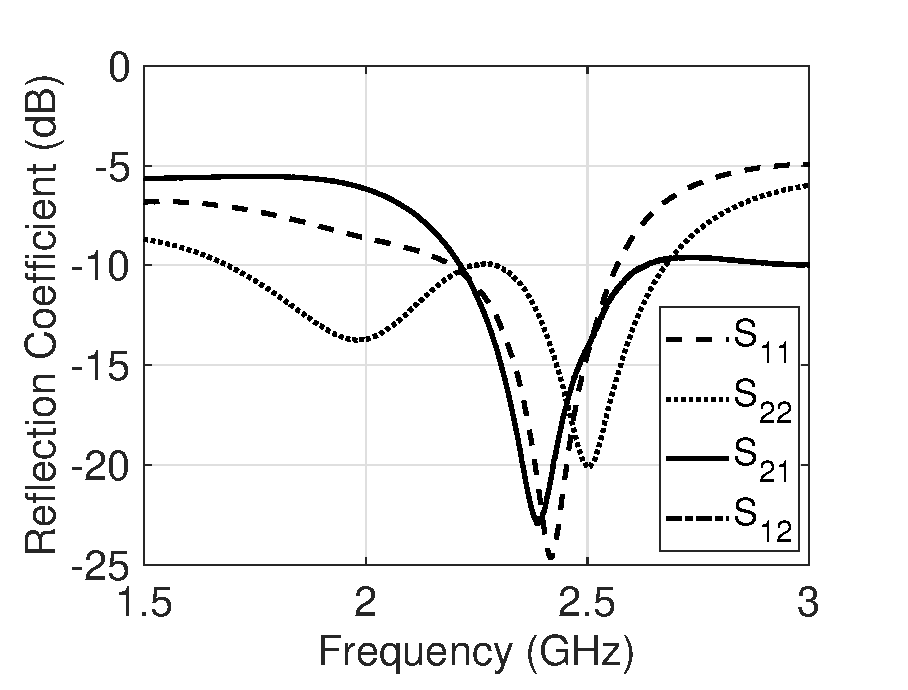
\includegraphics[width=0.9\columnwidth]{Figures/Fig4.eps}
\caption{S-parameters of ``single'' design. The VNA available input power ($P_\text{in,i}$) at each port was fixed at $-20$~dBm.}
\label{fig:S11_single}
\end{figure}


\begin{figure}[t]
\centering
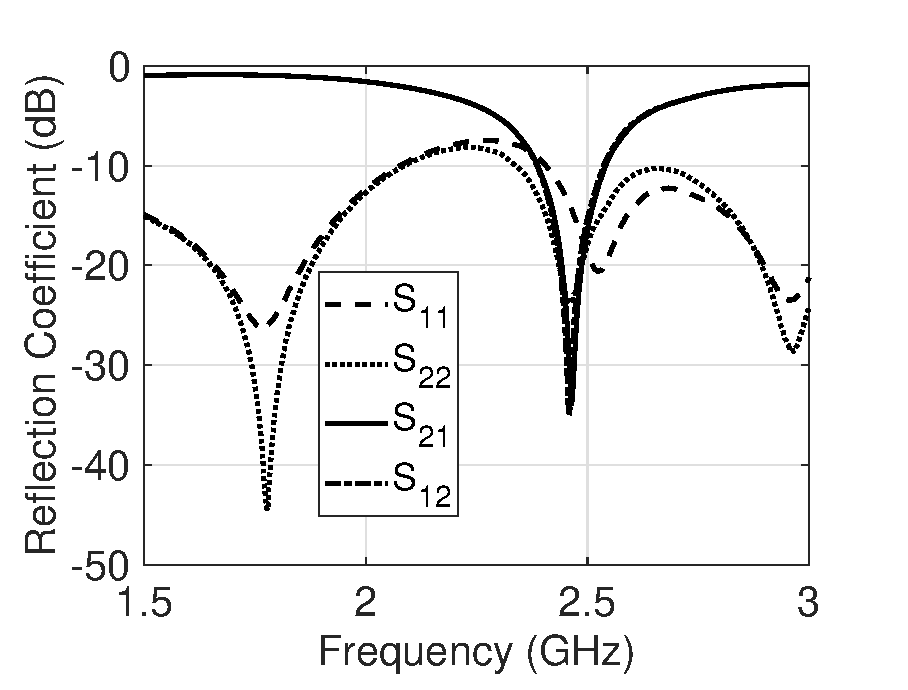
\includegraphics[width=0.9\columnwidth]{Figures/Fig5.eps}
\caption{S-parameters of ``double'' design. The VNA available input power ($P_\text{in,i}$) at each port was fixed at $-20$~dBm.}
\label{fig:S11_double}
\end{figure}



The  two converters were measured using a vector network analyser (VNA) at frequencies $1.5$~GHz to $3.5$~GHz.
%
The input signals were the carrier wave (CW) tones of VNA with $P_\text{in,1,2}= -20$~dBm.
%
The measured  S parameters of the ``single''  and ``double''  design  are   shown in Fig.~\ref{fig:S11_single} and Fig.~\ref{fig:S11_double}, respectively. 
%
It is shown that the reflection
coefficient at each port ($S_\text{11}$ and $S_\text{22}$) is bellow $-10$~dB at the center frequency of $2.4$~GHz. 

\begin{figure}[t]
\centering
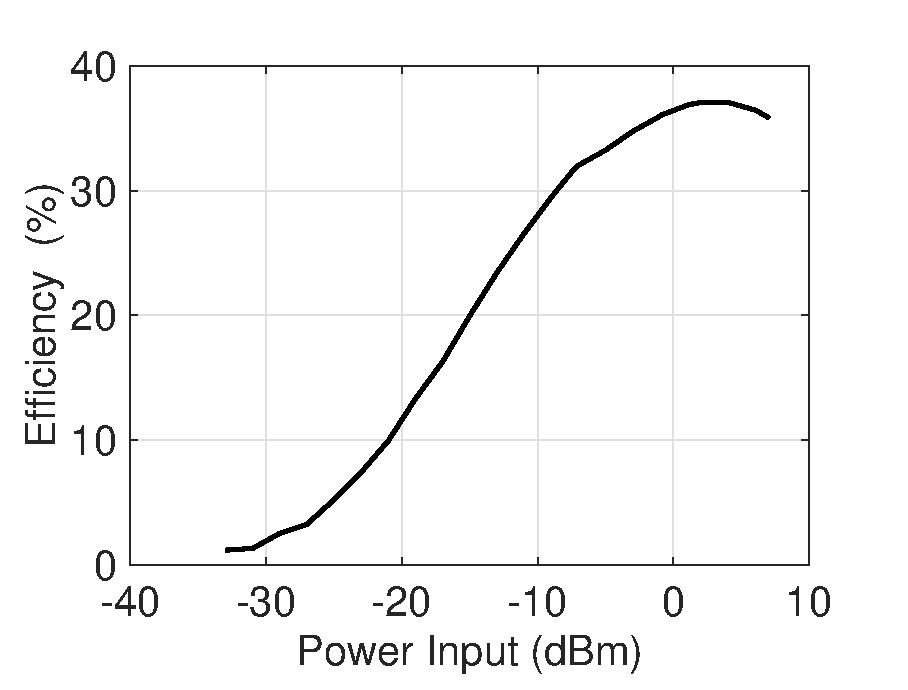
\includegraphics[width=0.9\columnwidth]{Figures/Fig6.eps}
\caption{Measurement rectifier efficiency of ``double'' design versus the available input power ($P_\text{in}$). The two input signals have the same phase at the frequency of $2.4$~GHz.}
\label{fig:eff_vs_pin}
\end{figure}
%
\begin{figure}[t]
\centering
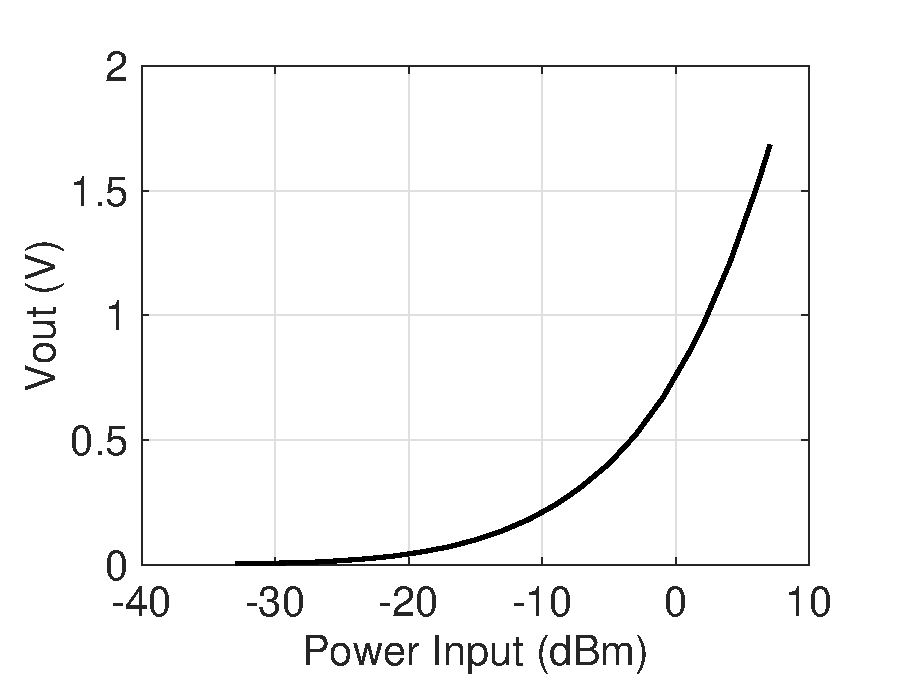
\includegraphics[width=0.9\columnwidth]{Figures/Fig7.eps}
\caption{Measured  output  voltage of ``double'' converter across the $1588~\Omega$ load.
The two input signals have the same phase at the frequency of $2.4$~GHz.}
\label{fig:vout_vs_pin}
\end{figure}
%
%
\begin{figure}[t]
\centering
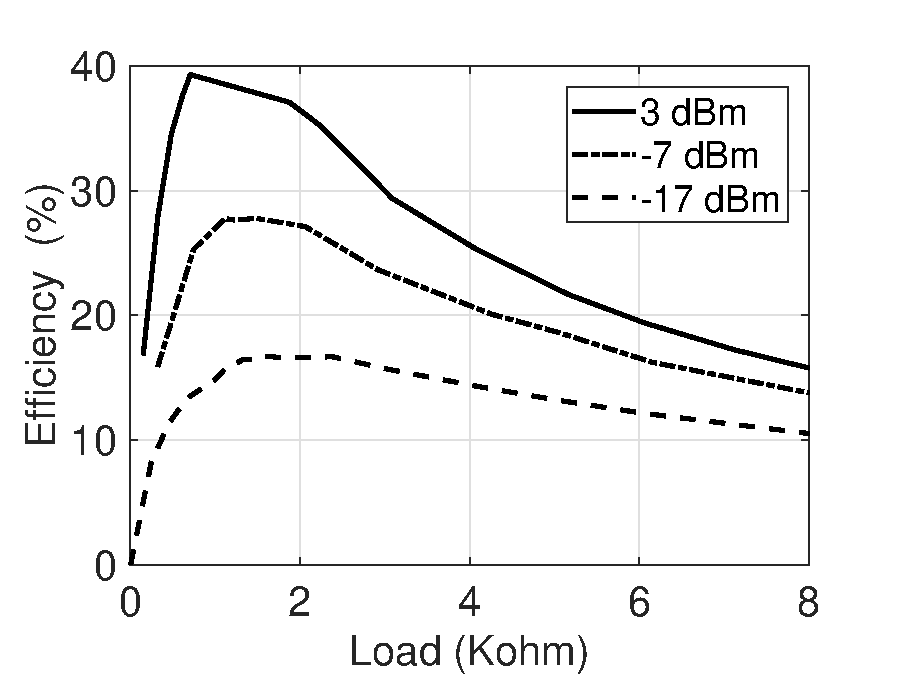
\includegraphics[width=0.9\columnwidth]{Figures/Fig11.eps}
\caption{Measured ``double'' rectifier efficiency versus load for different available input power at $2.4$~GHz.}
\label{fig:eff_vs_load_double}
\end{figure}
%
\begin{figure}[t]
\centering
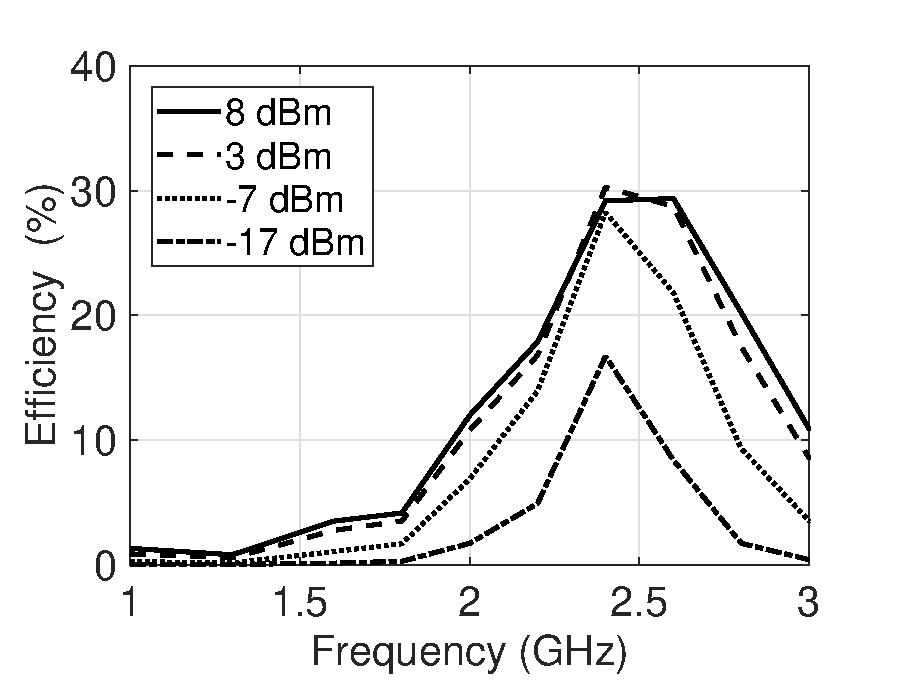
\includegraphics[width=0.9\columnwidth]{Figures/Fig12.eps}
\caption{Measured  ``double'' rectifier efficiency versus frequency for different power input levels. Load is fixed at $1559~\Omega$.}
\label{fig:eff_vs_freq_double}
\end{figure}
%
Regarding in-phase input RF signals, a commercial Wilkinson power divider was connected to a signal generator  for the efficiency measurements.
%
The divider outputs were connected with board inputs
through two ``same-length'' RF cables.
%
First,  a power meter (Keysight U8487A) was connected to each cable, measuring the received power of the signal. 
%
Next, the power meter was removed and cables were connected to the proposed ``double'' design.
%
The total power, $P_\text{in}$, is considered as the sum of $P_\text{in,1}$ and  $P_\text{in,2}$ which are the two divider output ports.
%
A voltmeter measures the voltage across the load, which is
fixed at  $1588~\Omega$. 
%
Fig.~\ref{fig:eff_vs_pin} depicts the measured results of $\eta$
versus  $P_\text{in}$ for the ``double'' design.
%
The efficiency is equal to $29.46\%$ and $9.93\%$ for $P_\text{in}$ equal to $-9$~dBm and $-21$~dBm, respectively.
%
The maximum  efficiency was achieved for $P_\text{in}=2$~dBm and it was found at $37\%$.
%
Fig.~\ref{fig:vout_vs_pin} shows the measured voltage values across the $1588~\Omega$  load. $V_\text{L}$ is equal with $51$~mV for  $P_\text{in}=-21$ dB and $240$~mV for $P_\text{in}=-9$~dBm, respectively.
%
%Fig.~\ref{fig:eff_vs_load_both_min17} shows the  efficiency of  ``single'' and ``double'' design  versus load for $P_\text{in}=-17$~dBm at $2.4$~GHz when the two inputs have zero phase difference (in-phase). 
%
Fig.~\ref{fig:eff_vs_load_double} presents the relation between the
efficiency and the load only for the ``double'' design using three power input levels, with the frequency fixed at $2.4$~GHz. 
%
In this case, a commercial potentiometer  was used for the load variation instead of a fixed resistor.
%
%It can be observed that the maximum $\eta$ occurs when $R_\text{L}\approx 1600~ \Omega$ for $P_\text{in}=-17$ dBm  as was expected from the simulation results.
%
It is obvious that there is a specific value for the load  that maximizes the efficiency for  each  $P_\text{in}$ value.
%
More specifically, for  $P_\text{in}=-7$~dBm  and  $P_\text{in}=3$~dBm, maximum efficiency is equal to $27.76 \%$ and $39.3\%$ for $1487~\Omega$ and $706~\Omega$ load, respectively.
%
For $P_\text{in}=-17$~dBm, the maximum efficiency occurs when $R_\text{L}\simeq1554~\Omega$ as was expected from the simulation results.
%
The measured efficiency versus frequency for different  $P_\text{in}$ and load fixed at $1554~\Omega$, is depicted in Fig.~\ref{fig:eff_vs_freq_double}.
%
It is shown that  ``double'' converter operates optimally at $2.4$~GHz for $P_\text{in}=-17$~dBm, as expected from the initial design. 
%
Also  the maximum efficiency is achieved at points very close to $2.4$~GHz for the rest of  power levels.
%
As can  observed from all above figures, there is a non-linear relation of the efficiency versus the  $P_\text{in}$, the frequency, as well as load  due to the diodes non-linearities.
%


\subsection{Out-of-Phase Input Measurements} 
\label{subsec:outof}

\begin{figure}[!t]
\centering
\includegraphics[width=0.9\columnwidth]{Figures/Fig13.eps}
\caption{Two signal generators measurement setup. The one  generator has a fixed  zero phase $2.4$~GHz signal. The second generator was used for the phase sweeping.}
\label{fig:setup}
\end{figure}
%
\begin{figure}[!t]
\centering
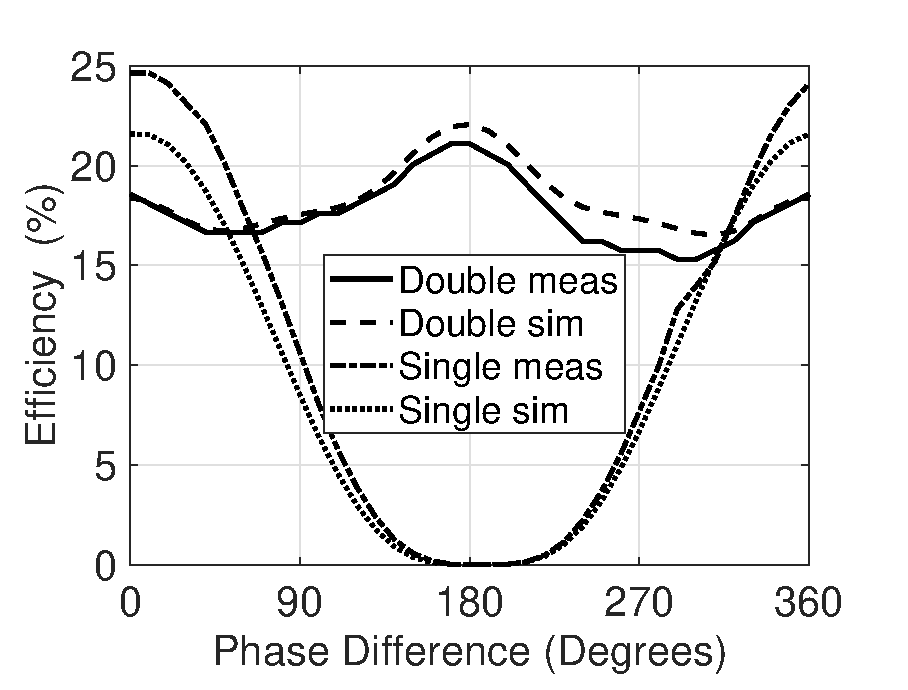
\includegraphics[width=0.9\columnwidth]{Figures/Fig14.eps}
\caption{Simulated and measured converter efficiency 
 versus phase difference at the input. 
 The  input signals had frequency $2.4$~GHz  with $P_\text{in}=-17$~dBm.}
\label{fig:eff_vs_phase_min17}
\end{figure}
%
\begin{figure}[t]
\centering
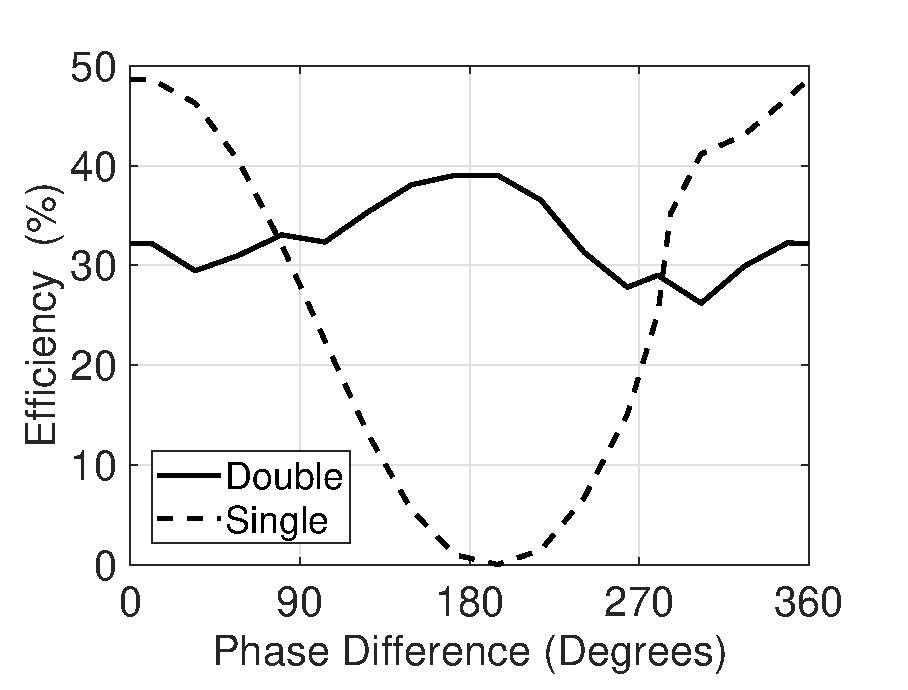
\includegraphics[width=0.9\columnwidth]{Figures/Fig15.eps}
\caption{Measured converter efficiency versus phase difference at the input.  The  input signals had frequency $2.4$~GHz  with $P_\text{in}=3$~dBm.}
\label{fig:eff_vs_phase_3}
\end{figure}
%


\begin{figure}[t]
\centering
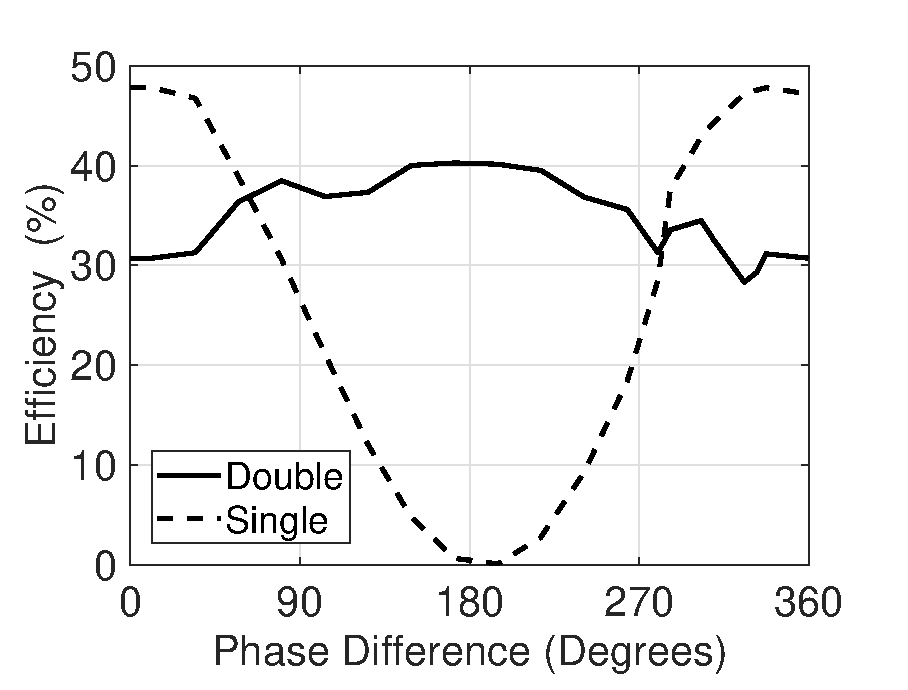
\includegraphics[width=0.9\columnwidth]{Figures/Fig16.eps}
\caption{Measured converter efficiency 
 versus phase difference at the input. 
 The  input signals had frequency $2.4$~GHz  with $P_{in}=8$~dBm. }
\label{fig:eff_vs_phase_8}
\end{figure}


Finally, the two designs were simulated and tested for input signals with different phase each one. 
%
Each board was connected with two synchronized signal
generators simultaneously as depicted in Fig.~\ref{fig:setup} setup.
%
The generator outputs were connected with boards 
through the same RF cables that were used in previous results. 
%
The first generator was used for
phase change from $0$ to $360$ degrees thus at the second generator,
the phase of the  signal was fixed at $0$ degrees.
%
In Fig.~\ref{fig:setup}  the voltmeter and the potentiometer are also depicted. %

Fig.~\ref{fig:eff_vs_phase_min17} shows the
efficiency achieved  for  $P_\text{in}=-17$~dBm and  phase difference from $0$ to $360$ degrees.
%
The load for ``double'' design was fixed at $1554~\Omega$ and for ``single'' at  $1759~\Omega$.
%
Very good agreement between simulation and measurements is
observed for both  designs. 
%
For the ``single''  design, the efficiency is maximized when the input signals are in-phase.
%
Moreover the efficiency goes to zero when the phase different is $180$ degrees and retreated periodically every $360$ degrees.
%
The ``double'' design addresses the problem  of the power dissipation on the isolation resistor and when the inputs signals are out of phase.
%
A constant efficiency it is observed between $15.31 \%$ and $21.9 \%$ from $0$ to $360$ degrees.
%
%It can be seen that the overall efficiency of the ``double'' converter is improved under all the phase difference conditions.
%
In  Fig.~\ref{fig:eff_vs_phase_3} the measured efficiency versus the phase difference for $P_\text{in}=3$~dBm  is depicted.
%
The optimal load for the ``double''  and ``single'' design was experimentally found at  $1022~\Omega$ and $909~\Omega$ respectively   based on the data shown in  Fig.~\ref{fig:eff_vs_load_double}.
%
The  topologies 
have similar behaviour for a  higher  $P_\text{in}$, as shown in  Fig.~\ref{fig:eff_vs_phase_min17}.   
%
The maximum efficiency of  ``double'' was measured at $39.02\%$ at $180$ degrees and the minimum  was $26.2\%$ at $300$ degrees.
%
Moreover the  ``single'' had maximum efficiency $48.61\%$ at zero degrees. 
%
Finally  the efficiency  for   $P_\text{in}=8$~dBm
is shown in Fig.~\ref{fig:eff_vs_phase_8}. 
%
The loads for   ``single''  and ``double'' designs were fixed at  $653~\Omega$ and  $774~\Omega$, respectively.
%
It can be observed that although the $P_\text{in}$ has been increased from $3$~dBm to $8$~dBm, the maximum efficiency cannot go over  $40\%$ for the ``double'' and over $47.8\%$ for the  ``single'' design, due to the breakdown  effect of the diodes. 
%


The number of diode elements in the circuit has a major influence on the output voltage of the energy harvesting circuit. 
%
Due to the fact that the diodes do not operate as ideal switches, when the number of diodes increases the total power dissipated in the diodes increases. 
%
This has an impact in the RF-to-dc conversation efficiency especially at low input power levels. Consequently, a rectifier circuit with one diode present a higher efficiency than a rectifier circuit with two diodes at low input power level \cite{nintanavongsa2012design}. 
%
This is also evident in Fig. 11 when the efficiency of the ``single'' design is higher than the efficiency of the ``double'' design.


\section{Discussion}
\label{sec:Discussion}
%
\begin{table}[t]
\renewcommand{\arraystretch}{1.1}
%% \extrarowheight as needed to properly center the text within the cells
\caption{RF-to-DC  Efficiency for Frequency $2.4$~GHz.}
\label{tab:Designs}
\centering 
\begin{tabular}{c||c||c||c||c}
\hline\hline  
      Work                              & Type & Ph. Diff. (Deg.) & Eff.   (\%) & $P_\text{in}$ (dBm)  \\
%                                        &               & (dBm)      (MHz) \\
\hline   \cite{lee2017hybrid}   & Rectifier & 0& $43\%$     &$-10$      \\
\hline   \cite{lee2017hybrid}   & Rectifier & 0& $10\%$     &$-17$      \\
\hline  \cite{sun2012design}            & Rectenna & 0& $50\%$       & $-17.2$    \\

\hline  \cite{georgiadis2010rectenna}   & Rectenna & 0& $38.2\%$     &$-19.2$      \\
\hline  \cite{georgiadis2010rectenna}   & Rectenna & 0& $15.3\%$     &$-9.2$      \\
\hline  \cite{vera2010design}   & Rectenna & 0& $15.7\%$     & $-20$    \\
\hline  \cite{vera2010design}   & Rectenna & 0& $42.1\%$     & $-10$    \\
\hline  \cite{olgun2010wireless}   & Rectenna & 0& $24\%$     &$-17$      \\
\hline  \cite{olgun2010wireless}   & Rectenna & 0& $55\%$     &$-7$      \\
\hline  \cite{curty2005remotely}   & Rectenna & 0& $37\%$     &$-25.7$      \\
\hline  \cite{chen2017maximum}   & Rectenna & 0& $31.8\%$     &$-15$      \\
\hline  This work                 & Rectifier & 0& $32\%$       & $-7$       \\
\hline  This work                 & Rectifier & 0& $18.5\%$       & $-17$       \\
\hline  This work                 & Rectifier & 180& $21.9\%$       & $-17$       \\
\hline  This work                 & Rectifier & 300& $15.3\%$       & $-17$       \\
%
\hline\hline
\end{tabular}
\end{table}
%
Table~\ref{tab:Designs}  offers
summary of achieved efficiency versus input power for various prior art designs operating at the $2.4$~GHz band.
%
We compare rectifiers/rectennas with our design for the in-phase conditions only, however it should be emphasized that our work focused on optimizing efficiency under non in-phase excitation. 
%
In order to further increase the efficiency, substrates with low losses \cite{sun2012design, georgiadis2010rectenna, vera2010design, olgun2010wireless} have been  proposed.
%
In \cite{sun2012design}, efficiency was increased to $50 \% $ for $ -17.2$~ dBm  input power level. 
%
A circular polarized rectenna was presented in \cite{georgiadis2010rectenna} with $15.3\%$ and $11.3\%$ efficiency for vertical and horizontal polarization, respectively. 
%
In \cite{vera2010design}, a dual polarized rectenna  consists of a square aperture coupled patch antenna and a rectifier circuit that was optimized at $2.45$~GHz with simulated efficiency $15.7\% $ at $-20$~dBm. 
%
In \cite{olgun2010wireless}  a  rectenna is proposed that is formed by a miniaturize $2^{nd}$ iteration Koch fractal patch antenna and a two-stage Dickson charge pump rectifier.
%
The rectenna achieves a small size with relatively high
realized gain ($4$~dBi) and good  conversion efficiency around $24\%$ at $-17$~dBm.
%
%In \cite{olgun2010wireless}, a similar work has been done by the same authors.
%
%The design is based on a Greinacher rectifier containing a $2\times2$ planar antenna array.
%
In \cite{curty2005remotely} a fully integrated remotely
powered  RFID chip  is described working at $2.45$~GHz. 
%
The necessary input power to operate the transponder is about $2.7~\mu$W.
%
The efficiency of the rectifier circuit is about $37\%$ for $-25.7$~dBm input power including the antenna effects.
%
In \cite{chen2017maximum}, an optimized rectenna structure is presented  which eliminates the matching circuit and exhibits the optimal rectifier architecture.
%
The antenna has been configured as an inductively-coupled-feed dipole and it is directly matched to the input impedance of the rectifier.
%
Can be noticed that all the above designs provide efficient  results only for in-phase signals.
 


In \cite{lee2017hybrid}  a  design approach for RF energy harvesting to receive more energy in a wide incident angle range is presented. 
%
A beam-forming matrix and a dc power management network  are used to the hybrid (RF and dc) power combining.
%
To experimentally verify the proposed hybrid combining array performance, four suspended patch antennas were attached to the RF energy harvesting architecture.
%
More specifically a $4\times 4$ Butler matrix and quadrature hybrids are used for
the beam-forming matrix in a hybrid power combining rectenna array. 
%
Each port of Butler matrix with $4\times 4$ array antenna has fixed  peak gain at a  fixed incident wave angle.

%
Instead of all the  designs,  the challenge for this work was to design an efficient rectification circuit, working in a wide incident angle range.
%
Our design uses the minimum number of inputs and discrete lumped elements  in order to maintain a constant RF-to-dc efficiency over a wide angular range compared to the other designs of table~\ref{tab:Designs}.  




\section{Conclusion \& Future Work}
\label{sec:Conclusion}
%
In this work, we present a rectifier  circuit for RF energy harvesting. 
%
%The RF-to-dc converter consists of a Wilkinson combiner and two single rectifier circuits in order to collect the energy from two inputs when the phase difference between them is not zero. 
%
%Using the proposed modified Wilkinson power combiner by replacing the isolation resistor with a single rectifier, 
%
%the power originally lost in the isolation resistor can be recycled to improve the overall efficiency.
%
%
%demonstrating high efficiency rectification, for low input power.
%
Our rectifier combiner do RF power combining and dc power combining in order to achieve a high conversion efficiency with minimum variation from RF signals with arbitrary phase, thereby maintaining both a high gain and an omnidirectional characteristic for a rectenna.
%
A prototype was fabricated on  low-cost FR-4 substrate and measurements agreed with simulations.
%tem times  
%
%
%Finally, we could have isotropic antennas (e.g. monopoles) that  could harvest energy from all angles with high efficiency.

Nowadays, one of  the major research goals is to overcome fundamental challenges related to the miniaturization of  electronic circuits  in order to scale them up  in mmWave frequencies.
%
The  mmWave communications is a key candidate technology for future 5G cellular networks. 
%
This is mainly due to the availability of large spectrum resources at higher frequencies, which leads to much higher data rates.
%
Transferring wireless energy, in mmWave frequencies seems attractive for future applications where base stations with 
directional beamforming capabilities could supply miniaturized low-power devices like RFID tags.
%
The base station/reader could align its  narrow beams with the tags in order to supply them with power
and the same  signals could  be also used for the communication links. 
%
The proposed system could be miniaturized and applied on passive RFID tag implementations in order to collect energy from multiple directions.
%
Our novel circuit could be also combined with a retro-directive antenna array such a Van Atta array
in order  to reradiate the signal 
back to the reader \cite{miyamoto2002retrodirective, cespedes2012retro, braaten2015compact} and at the same time harvest a maximum amount of power independently of the angle of arrival of the incoming reader signal. 

\section*{Acknowledgment}
\normalsize
The authors  would like
to thank LRF and ICON. The authors would like to thank also
all members of Microwaves and Antenna Engineering Research
Group, Heriot-Watt University, Edinburgh, Scotland,
UK, EH14 4AS for their help in various steps throughout this
work.

% Generated by IEEEtran.bst, version: 1.14 (2015/08/26)
\begin{thebibliography}{10}
\providecommand{\url}[1]{#1}
\csname url@samestyle\endcsname
\providecommand{\newblock}{\relax}
\providecommand{\bibinfo}[2]{#2}
\providecommand{\BIBentrySTDinterwordspacing}{\spaceskip=0pt\relax}
\providecommand{\BIBentryALTinterwordstretchfactor}{4}
\providecommand{\BIBentryALTinterwordspacing}{\spaceskip=\fontdimen2\font plus
\BIBentryALTinterwordstretchfactor\fontdimen3\font minus
  \fontdimen4\font\relax}
\providecommand{\BIBforeignlanguage}[2]{{%
\expandafter\ifx\csname l@#1\endcsname\relax
\typeout{** WARNING: IEEEtran.bst: No hyphenation pattern has been}%
\typeout{** loaded for the language `#1'. Using the pattern for}%
\typeout{** the default language instead.}%
\else
\language=\csname l@#1\endcsname
\fi
#2}}
\providecommand{\BIBdecl}{\relax}
\BIBdecl

\bibitem{shinohara2011power}
N.~Shinohara, ``Power without wires,'' \emph{{IEEE} Microw. Mag.}, vol.~12,
  no.~7, pp. S64--S73, Dec. 2011.

\bibitem{pinuela2013ambient}
M.~Pi{\~n}uela, P.~D. Mitcheson, and S.~Lucyszyn, ``Ambient {RF} energy
  harvesting in urban and semi-urban environments,'' \emph{{IEEE} Trans.
  Microw. Theory Techn.}, vol.~61, no.~7, pp. 2715--2726, May 2013.

\bibitem{niotaki2014solar}
K.~Niotaki, A.~Collado, A.~Georgiadis, S.~Kim, and M.~M. Tentzeris,
  ``Solar/{E}lectromagnetic energy harvesting and wireless power
  transmission,'' \emph{Proc. {IEEE}}, vol. 102, no.~11, pp. 1712--1722, Nov.
  2014.

\bibitem{kim2014ambient}
S.~Kim, R.~Vyas, J.~Bito, K.~Niotaki, A.~Collado, A.~Georgiadis, and M.~M.
  Tentzeris, ``Ambient {RF} energy-harvesting technologies for self-sustainable
  standalone wireless sensor platforms,'' \emph{Proc. {IEEE}}, vol. 102,
  no.~11, pp. 1649--1666, Nov. 2014.

\bibitem{brown1984history}
W.~C. Brown, ``The history of power transmission by radio waves,'' \emph{{IEEE}
  Trans. Microw. Theory Techn.}, vol.~32, no.~9, pp. 1230--1242, 1984.

\bibitem{valenta2014harvesting}
C.~R. Valenta and G.~D. Durgin, ``Harvesting wireless power: Survey of
  energy-harvester conversion efficiency in far-field, wireless power transfer
  systems,'' \emph{{IEEE} Microw. Mag.}, vol.~15, no.~4, pp. 108--120, May
  2014.

\bibitem{assimonis2015sensitive}
S.~D. Assimonis, S.~N. Daskalakis, and A.~Bletsas, ``Sensitive and efficient
  {RF} harvesting supply for batteryless backscatter sensor networks,''
  \emph{{IEEE} Trans. Microw. Theory Techn.}, vol.~64, no.~4, pp. 1327--1338,
  Apr. 2016.

\bibitem{kotani2009high}
K.~Kotani, A.~Sasaki, and T.~Ito, ``High-efficiency differential-drive {CMOS}
  rectifier for {UHF RFID}s,'' \emph{{IEEE} J. of Solid-State Circuits},
  vol.~44, no.~11, pp. 3011--3018, Nov. 2009.

\bibitem{kimionis2017millimeter}
J.~Kimionis, A.~Georgiadis, and M.~M. Tentzeris, ``Millimeter-wave backscatter:
  A quantum leap for gigabit communication, {RF} sensing, and wearables,'' in
  \emph{Proc. {IEEE} MTT-S Int. Microw. Symp. (IMS)}, Honolulu, HI, USA, Jun.
  2017, pp. 812--815.

\bibitem{tong2019achieving}
T.-H. Lin, S.~Daskalakis, A.~Georgiadis, and M.~M. Tentzeris, ``Achieving fully
  autonomous system-on-package designs: An embedded-on-package {5G} energy
  harvester within {3D} printed multilayer flexible packaging structures,'' in
  \emph{Proc. {IEEE} MTT-S Int. Microw. Symp. (IMS)}, Boston, MA, USA, Jun.
  2019.

\bibitem{hester2017mm}
J.~Hester and M.~M. Tentzeris, ``A mm-wave ultra-long-range energy-autonomous
  printed {RFID}-enabled {V}an-{A}tta wireless sensor: At the crossroads of
  {5G} and {I}o{T},'' in \emph{Proc. {IEEE} MTT-S Int. Microw. Symp. (IMS)},
  Honololu, HI, USA, Jun. 2017.

\bibitem{marshall2013staggered}
B.~R. Marshall and G.~D. Durgin, ``Staggered pattern charge collection: Antenna
  technique to improve {RF} energy harvesting,'' in \emph{Proc. {IEEE} Int.
  Conf. on RFID}, Penang, Malaysia, May 2013, pp. 30--35.

\bibitem{lee2017hybrid}
D.-J. Lee, S.-J. Lee, I.-J. Hwang, W.-S. Lee, and J.-W. Yu, ``Hybrid power
  combining rectenna array for wide incident angle coverage in {RF} energy
  transfer,'' \emph{{IEEE} Trans. Microw. Theory Techn.}, vol.~65, no.~9, pp.
  3409--3418, Mar. 2017.

\bibitem{olgun2010low}
U.~Olgun, C.-C. Chen, and J.~L. Volakis, ``Low-profile planar rectenna for
  batteryless {RFID} sensors,'' in \emph{Proc. {IEEE} Antennas and Prop.
  Society Int. Symp.}, Toronto, ON, Canada, Sep. 2010, pp. 1--4.

\bibitem{alneyadi20142}
F.~Alneyadi, M.~Alkaabi, S.~Alketbi, S.~Hajraf, and R.~Ramzan, ``2.4 {GH}z
  {WLAN} {RF} energy harvester for passive indoor sensor nodes,'' in
  \emph{Proc. {IEEE} Int. Conf. on Semiconductor Electronics (ICSE)}, Kuala
  Lumpur, Malaysia, Oct. 2014, pp. 471--474.

\bibitem{wangpower}
T.~H. Wang and J.~H. Chen, ``Power recycling using {W}ilkinson power combiner
  with pulsewidth modulation,'' in \emph{Proc. {IEEE} Int. Symp. on Radio-Freq.
  Integr. Tech. (RFIT)}, Seoul, South Korea, Sep. 2017.

\bibitem{daskalakis20182}
S.~N. Daskalakis, G.~Goussetis, and A.~Georgiadis, ``A 2.4 {GH}z rectifier
  insensitive to the angle of incidence of incoming waves,'' in \emph{Proc.
  {IEEE} 2nd URSI Atlantic Radio Science Meeting (AT-RASC)}, Gran Canaria,
  Spain, May-Jun. 2018, pp. 1--4.

\bibitem{wilkinson1960n}
E.~J. Wilkinson, ``An {N}-way hybrid power divider,'' \emph{{IEEE} IRE Trans.
  Microw. Theory Techn.}, vol.~8, no.~1, pp. 116--118, Jan. 1960.

\bibitem{nintanavongsa2012design}
P.~Nintanavongsa, U.~Muncuk, D.~R. Lewis, and K.~R. Chowdhury, ``Design
  optimization and implementation for {RF} energy harvesting circuits,''
  \emph{{IEEE} J. on Emerg. and Select. Topics in Circuits and Systems},
  vol.~2, no.~1, pp. 24--33, Mar. 2012.

\bibitem{boaventura2013optimum}
A.~Boaventura, A.~Collado, N.~B. Carvalho, and A.~Georgiadis, ``Optimum
  behavior: Wireless power transmission system design through behavioral models
  and efficient synthesis techniques,'' \emph{{IEEE} Microw. Mag.}, vol.~14,
  no.~2, pp. 26--35, 2013.

\bibitem{SMS7630}
\BIBentryALTinterwordspacing
\emph{SMS7630 Surface-Mount Mixer and Detector Schottky Diodes, product
  manual}, Skyworks, Inc., 2018. [Online]. Available:
  \url{http://www.skyworksinc.com/uploads/documents/Surface_Mount_Schottky_Diodes_200041AD.pdf}
\BIBentrySTDinterwordspacing

\bibitem{pournoori2018rf}
N.~Pournoori, M.~W.~A. Khan, L.~Ukkonen, and T.~Bj{\"o}rninen, ``{RF} energy
  harvesting system with {RFID}-enabled charge storage monitoring,'' in
  \emph{Proc. {IEEE} Conf. on RFID Techn. and Appl. (RFID-TA)}, Macau, China,
  Sep. 2018, pp. 1--5.

\bibitem{sun2012design}
H.~Sun, Y.-x. Guo, M.~He, and Z.~Zhong, ``Design of a high-efficiency
  2.45-{GHz} rectenna for low-input-power energy harvesting,'' \emph{{IEEE}
  Antennas Wireless Propag. Lett.}, vol.~11, pp. 929--932, Aug. 2012.

\bibitem{georgiadis2010rectenna}
A.~Georgiadis, G.~Andia, and A.~Collado, ``Rectenna design and optimization
  using reciprocity theory and harmonic balance analysis for electromagnetic
  ({EM}) energy harvesting,'' \emph{{IEEE} Antennas Wireless Propag. Lett.},
  vol.~9, pp. 444--446, May 2010.

\bibitem{vera2010design}
G.~A. Vera, A.~Georgiadis, A.~Collado, and S.~Via, ``Design of a 2.45 {GHz}
  rectenna for electromagnetic {(EM)} energy scavenging,'' in \emph{Proc.
  {IEEE} Radio and Wireless Symp. (RWS)}, New Orleans, LA, USA, Mar. 2010, pp.
  61--64.

\bibitem{olgun2010wireless}
U.~Olgun, C.-C. Chen, and J.~L. Volakis, ``Wireless power harvesting with
  planar rectennas for 2.45 {GHz} {RFID}s,'' in \emph{Proc. {IEEE} URSI Int.
  Symp on Electromagnetic Theory (EMTS)}, Berlin, Germany, Aug. 2010, pp.
  329--331.

\bibitem{curty2005remotely}
J.-P. Curty, N.~Joehl, C.~Dehollain, and M.~J. Declercq, ``Remotely powered
  addressable {UHF} {RFID} integrated system,'' \emph{{IEEE} J. of Solid-State
  Circuits}, vol.~40, no.~11, pp. 2193--2202, Oct. 2005.

\bibitem{chen2017maximum}
Y.-S. Chen and C.-W. Chiu, ``Maximum achievable power conversion efficiency
  obtained through an optimized rectenna structure for {RF} energy
  harvesting,'' \emph{{IEEE} Trans. on Antennas and Propagation.}, vol.~65,
  no.~5, pp. 2305--2317, Mar. 2017.

\bibitem{miyamoto2002retrodirective}
R.~Y. Miyamoto and T.~Itoh, ``Retrodirective arrays for wireless
  communications,'' \emph{{IEEE} Microw. Mag.}, vol.~3, no.~1, pp. 71--79, Aug.
  2002.

\bibitem{cespedes2012retro}
J.~Cespedes, F.~Giuppi, A.~Collado, and A.~Georgiadis, ``A retro-directive
  {UHF} {RFID} tag on paper substrate,'' in \emph{Proc. {IEEE} Conf. on RFID
  Techn. and Appl. (RFID-TA)}, Nice, France, Nov. 2012, pp. 263--266.

\bibitem{braaten2015compact}
B.~D. Braaten, S.~Asif, S.~Khan, J.~Hansen, and D.~L. Ewert, ``A compact
  printed {V}an {A}tta {A}rray with zero-phase {CRLH} transmission lines,'' in
  \emph{Proc. {IEEE} Antennas and Prop. Society Int. Symp.}, Vancouver, BC,
  Canada, Jul. 2015, pp. 1856--1857.

\end{thebibliography}


%%%%%%%%%%%%%%%%%%%%%%%%%%%%%%%%%%%%%%%%%%%%%
\begin{IEEEbiography}[{
\includegraphics[width=1in,height=1.55in,clip,keepaspectratio]{Figures/Fig17.png}}]
{Spyridon Nektarios Daskalakis} (S'12) was born in Heraklion, Greece in 1991. He received with excellence his Engineering Diploma and the M.Sc. in Electrical and Computer Engineering from Technical University of Crete (TUC) in 2014 and 2016, respectively. He is currently working toward the PhD degree in School of Engineering and Physical Sciences from Heriot-Watt university, Edinburgh UK. 

His current research interests include low-power, low-cost wireless sensor networks and energy harvesting. Particularly he focuses on backscatter radio communication, batteryless sensors, low cost software-defined radio, environmental sensing and RF energy harvesting. 
He has received fellowship award by the Clinton Global Initiative University 2014 (USA), the Onassis Foundation (graduate studies 2015/16 scholarship), the Lloyds Register Foundation (LRF) and the International Consortium in Nanotechnology (ICON). He was a recipient for two short-term scientific mission grands from COST Action IC1301 WiPE in School of Electrical and Computer Engineering, Georgia Institute of Technology, Atlanta in 2016, and the Centre Tecnològic de Telecomunicacions de Catalunya, Barcelona in 2015. 
He  is also a recipient  of MTT-S Graduate Fellowship for 2019 from IEEE Microwave Theory and Techniques Society.
He has been a member of the IEEE Microwave Theory and Techniques Society, the IEEE Council on RFID and the IEEE Sensors Council.
\end{IEEEbiography}

\begin{IEEEbiography}[{
\includegraphics[width=1in,height=1.55in,clip,keepaspectratio]{Figures/Fig18.jpg}}]
{Apostolos Georgiadis} (S'94-M'02-SM'08) was
born in Thessaloniki, Greece. He received the B.S.
degree in physics and M.S. degree in telecommunications
from the Aristotle University of Thessaloniki,
Thessaloniki, Greece, in 1993 and 1996,
respectively, and the Ph.D. degree in electrical
engineering from the University of Massachusetts,
Amherst, MA, USA, in 2002.

In 2002, he joined Global Communications
Devices, North Andover, MA, USA, as a Systems
Engineer where he involved in CMOS transceivers
for wireless network applications. In 2003, he joined Bermai Inc., Minnetonka,
MN, USA, as an RF/Analog Systems Architect. In 2005, he joined the
University of Cantabria, Santander, Spain, as a Juan de la Cierva Fellow
Researcher. In 2006, he was a consultant for Bitwave Semiconductor, Lowell,
MA, USA. He collaborated with ACORDE S.A., Santander, Spain, where
he was involved in the design of integrated CMOS VCOs for ultra-wideband
applications. In 2007, he joined the Technological Telecommunications Center
of Catalonia (CTTC), Spain, as a Senior Researcher of communications
subsystems. From 2013 to 2016, he was a Group Leader with the Microwave
Systems and Nanotechnology Department, CTTC. In 2016, he joined Heriot-Watt University, Edinburgh, U.K., as an Associate Professor. He has authored
more than 180 papers in peer-reviewed journals and international conferences.
His current research interests include energy harvesting and wireless power
transmission, RFID technology, active antennas and phased-array antennas,
inkjet and 3-D printed electronics, millimeter-wave systems.

Dr. Georgiadis was a recipient of the Fulbright Scholarship for graduate studies at the University of Massachusetts, in 1996. He was the General Chair of the 2011 IEEE RFID-TA Conference and the General Co-Chair of the 2011 IEEE MTT-S IMWS on Millimeter Wave Integration Technologies. He is an EU Marie Curie Global Fellow. He is member of the IEEE MTT-S TC-24 RFID Technologies (past Chair) and a member of the IEEE MTT-S TC-26 Wireless Energy Transfer and Conversion. He was an Associate Editor of the IET Microwaves Antennas and Propagation journal, IEEE MICROWAVE AND WIRELESS COMPONENTS LETTERS, and the IEEE RADIO FREQUENCY IDENTIFICATION (RFID) VIRTUAL JOURNAL. He serves as an Associate Editor for the IEEE JOURNAL OF RFID and is the Founder and the Editor-in-Chief of the Wireless Power Transfer Journal of Cambridge University Press. He is the Chair of the URSI Commission D, Electronics, and Photonics, and an AdCom member of the IEEE Council on RFID serving as the Vice President of conferences. He is a Distinguished Lecturer of the IEEE Council on RFID. In 2016, his proposal for Inkjet/3-D printed millimeter-wave systems received the Bell Labs Prize, third place among more than 250 proposals recognizing ideas that ``change the game" in the field of information and communications technologies.
\end{IEEEbiography}
%%%%%%%%%%%%%%%%%%%%%%%%%%%%%%%%%%%%%%%%%%%%%%%%%%%%%%%%%
\begin{IEEEbiography}[{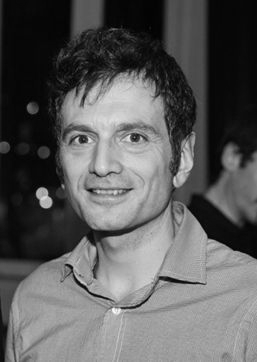
\includegraphics[width=0.95in,height=1.55in,clip,keepaspectratio]{Figures/Fig19.png}}]
{George Goussetis} (S'99-M'02-SM'12) received the Diploma degree in Electrical and Computer Engineering from the National Technical University of Athens, Greece, in 1998, and the Ph.D. degree from the University of Westminster, London, UK, in 2002. In 2002 he also graduated B.Sc. in physics (first class) from University College London (UCL), UK. 

In 1998, he joined the Space Engineering, Rome, Italy, as RF Engineer and in 1999 the Wireless Communications Research Group, University of Westminster, UK, as a Research Assistant. Between 2002 and 2006 he was a Senior Research Fellow at Loughborough University, UK. He was a Lecturer (Assistant Professor) with Heriot-Watt University, Edinburgh, UK between 2006 and 2009 and a Reader (Associate Professor) with Queen’s University Belfast, UK, between 2009 and 2013. In 2013 he joined Heriot-Watt as a Reader and was promoted to Professor in 2014, where he currently directs the Institute of Sensors Signals and Systems. He has authored or co-authored over 500 peer-reviewed papers five book chapters one book and four patents. His research interests are in the area of microwave and antenna components and subsystems. 

Dr. Goussetis has held a research fellowship from the Onassis foundation in 2001, a research fellowship from the UK Royal Academy of Engineering between 2006-2011 and European Marie-Curie experienced researcher fellowships in 2011-12 and again in 2014-17. He is the co-recipient of the 2011 European Space Agency young engineer of the year prize, the 2011 EuCAP best student paper prize, the 2012 EuCAP best antenna theory paper prize and the 2016 Bell Labs prize. He has served as Associate Editor to the IEEE Antennas and Wireless Propagation Letters.

\end{IEEEbiography}


%%%%%%%%%%%%%%%%%%%%%%%%%%%%%%%%%%%%%
\begin{IEEEbiography}[{
\includegraphics[width=1in,height=1.55in,clip,keepaspectratio]{Figures/Fig20.jpg}}]
{Manos M. Tentzeris}  (S'89-M'98-SM'03-F'10) received the Diploma Degree in Electrical and Computer Engineering from the National Technical University of Athens (``Magna Cum Laude") in Greece and the M.S. and Ph.D. degrees in Electrical Engineering and Computer Science from the University of Michigan, Ann Arbor, MI and he is currently Ken Byers Professor in Flexible Electronics with School of ECE, Georgia Tech, Atlanta, GA

He has published more than 650 papers in refereed Journals and Conference Proceedings, 5 books and 25 book chapters. Dr. Tentzeris has helped develop academic programs in 3D/inkjet-printed RF electronics and modules, flexible electronics, origami and morphing electromagnetics, Highly Integrated/Multilayer Packaging for RF and Wireless Applications using ceramic and organic flexible materials, paper-based RFID's and sensors, wireless sensors and biosensors, wearable electronics, ``Green" electronics, energy harvesting and wireless power transfer, nanotechnology applications in RF, Microwave MEM's, SOP-integrated (UWB, multiband, mmW, conformal) antennas and heads the ATHENA research group (20 researchers). He has served as the Head of the GT-ECE Electromagnetics Technical Interest Group, as the Georgia Electronic Design Center Associate Director for RFID/Sensors research and as the Georgia Tech NSF-Packaging Research Center Associate Director for RF Research and the RF Alliance Leader.  He was the recipient/co-recipient of the 2017 Georgia Tech Outstanding Achievement in Research Program Development Award, 2016 Bell Labs Award Competition 3rd Prize, the 2015  IET Microwaves, Antennas and Propagation Premium Award, the 2014 Georgia Tech ECE Distinguished Faculty Achievement Award, the 2014 IEEE RFID-TA Best Student Paper Award, the 2013 IET Microwaves, Antennas and Propagation Premium Award, the 2012 FiDiPro Award in Finland, the iCMG Architecture Award of Excellence, the 2010 IEEE Antennas and Propagation Society Piergiorgio L. E. Uslenghi Letters Prize Paper Award, the 2011 International Workshop on Structural Health Monitoring Best Student Paper Award, the 2010 Georgia Tech Senior Faculty Outstanding Undergraduate Research Mentor Award,  the 2009 IEEE Transactions on Components and Packaging Technologies Best Paper Award, the 2009 E.T.S. Walton Award from the Irish Science Foundation, the 2007 IEEE APS Symposium Best Student Paper Award, the 2007 IEEE IMS Third Best Student Paper Award, the 2007 ISAP 2007 Poster Presentation Award, the 2006 IEEE MTT Outstanding Young Engineer Award, the 2006 Asian-Pacific Microwave Conference Award, the 2004 IEEE Transactions on Advanced Packaging Commendable Paper Award, the 2003 NASA Godfrey ``Art" Anzic Collaborative Distinguished Publication Award, the 2003 IBC International Educator of the Year Award, the 2003 IEEE CPMT Outstanding Young Engineer Award, the 2002 International Conference on Microwave and Millimeter-Wave Technology Best Paper Award (Beijing, CHINA), the 2002 Georgia Tech-ECE Outstanding Junior Faculty Award, the 2001 ACES Conference Best Paper Award and the 2000 NSF CAREER Award and the 1997 Best Paper Award of the International Hybrid Microelectronics and Packaging Society. He was the TPC Chair for IEEE IMS 2008 Symposium and the Chair of the 2005 IEEE CEM-TD Workshop and he is the Vice-Chair of the RF Technical Committee (TC16) of the IEEE CPMT Society. He is the founder and chair of the RFID Technical Committee (TC24) of the IEEE MTT Society and the Secretary/Treasurer of the IEEE C-RFID. 

He is the Associate Editor of IEEE Transactions on Microwave Theory and Techniques, IEEE Transactions on Advanced Packaging and International Journal on Antennas and Propagation. 
Dr. Tentzeris was a Visiting Professor with the Technical University of Munich, Germany for the summer of 2002, a Visiting Professor with GTRI-Ireland in Athlone, Ireland for the summer of 2009 and a Visiting Professor with LAAS-CNRS in Toulouse, France for the summer of 2010. He has given more than 100 invited talks to various universities and companies all over the world. He is a Fellow of IEEE, a member of URSI-Commission D, a member of MTT-15 committee, an Associate Member of EuMA, a Fellow of the Electromagnetic Academy and a member of the Technical Chamber of Greece. Prof. Tentzeris served as one of the IEEE MTT-S Distinguished Microwave Lecturers from 2010-2012 and he is one of the IEEE CRFID Distinguished Lecturers.
\end{IEEEbiography}

%%%%%%%%%%%%%%%%%%%%%%%%%%%%%%%%%%%%%


%\vspace*{-2\baselineskip}
%%%%%%%%%%%%%%%%%%%%%%%%%%%%%%%%%%%%%


% that's all folks


\end{document}


